% =====================================================================
%  riesgos.tex
%  Sección 6 — Plan de gestión de riesgos asociado a los requisitos.
%  Aplica el proceso del capítulo 9 de referencia (identificar, analizar,
%  evaluar y tratar el riesgo en cada etapa de la ingeniería de
%  requisitos) al catálogo de RedPepper.
%  Las tablas de registro, ranking y plan se generan desde
%  plantillas/registro_riesgos.csv con scripts/generar_riesgos.py.
% =====================================================================

% =====================================================================
%  riesgos-macros.tex — GENERADO AUTOMÁTICAMENTE
%  Fuente: plantillas/registro_riesgos.csv
%  Regenerar con: python3 scripts/generar_riesgos.py  (o make riesgos)
%  No editar a mano: cualquier cambio se pierde al regenerar.
% =====================================================================
% Macros e indicadores calculados por scripts/generar_riesgos.py
\newcommand{\RiesgosTotal}{30}
\newcommand{\RiesgosResueltos}{1}
\newcommand{\RiesgosEnProceso}{10}
\newcommand{\RiesgosPendientes}{16}
\newcommand{\RiesgosRetrasados}{3}
\newcommand{\RiesgosCriticos}{2}
\newcommand{\RiesgosAltos}{7}
\newcommand{\RiesgosMedios}{17}
\newcommand{\RiesgosBajos}{4}
\newcommand{\RiesgosAbiertos}{29}
\newcommand{\ExposicionTotal}{135\,415}
\newcommand{\ColchonBruto}{35,15}
\newcommand{\ColchonResidual}{15,05}
\newcommand{\ColchonAhorro}{20,1}
\newcommand{\ColchonPorcentaje}{43,9}
\newcommand{\ColchonResidualPorcentaje}{18,8}
\newcommand{\JornadasProyecto}{80}


\clearpage
\section{Plan de gestión de riesgos asociado a los requisitos}
\label{sec:riesgos}

\noindent{\small\textbf{Versión 1} \textperiodcentered{} avance para la
revisión del 26 de noviembre de 2026 \textperiodcentered{} cuantificación
preliminar sujeta a validación con el equipo y con el interesado.}\par\vspace{0.5em}

\subsection{Propósito y alcance}
\label{subsec:riesgos-proposito}

La ingeniería de requisitos se mueve entre lo informal de la necesidad y lo
formal de la especificación. En ese tránsito, el riesgo no es una amenaza
que deba evitarse: es una condición incierta que, si no se trata a tiempo,
se convierte en un defecto de concepción, en un retrabajo o en un requisito
de calidad descubierto cuando el producto ya está en producción. Esta
sección operacionaliza esa idea, siguiendo el proceso del capítulo 9
\enquote{Gestión del riesgo en los requisitos} de Huertas Niquén, Pérez Vera
y Cabrera Málaga, sobre el catálogo de RedPepper: identifica
los riesgos asociados a los requisitos, los analiza en probabilidad e
impacto, los evalúa con un índice cuantitativo y define el tratamiento de
los diez más severos.

El alcance es acotado y explícito. Se trabaja sobre los requisitos de las
secciones anteriores (52 fichas de educción, 52 cadenas de ilación, 20 RF,
8 RNF y 39 derivados candidatos), no sobre el proyecto completo: los riesgos
de cronograma, presupuesto, proveedores o personal se recogen solo en
cuanto afectan la definición de un requisito. La unidad de registro es el
requisito, identificado con su código de ficha (\texttt{EDU-},
\texttt{ILA-}) o con el código del requisito especificado (\texttt{RF-},
\texttt{RNF-}, \texttt{R-}) y numerado con el prefijo \texttt{R-} para el
seguimiento.

\paragraph{Resumen ejecutivo.} El avance deja cuatro resultados
verificables:

\begin{itemize}
  \item Se identificaron y registraron \RiesgosTotal{} riesgos, distribuidos
  en las tres etapas: nueve en educción, ocho en ilación y trece en
  especificación (Tabla~\ref{tab:riesgos-resumen}).
  \item Hay \RiesgosCriticos{} riesgos críticos y \RiesgosAltos{} altos según
  el índice P-I; solo \RiesgosResueltos{} está cerrado y \RiesgosAbiertos{}
  siguen abiertos.
  \item La exposición total estimada asciende a S/\,\ExposicionTotal{} y el
  colchón de exposición bruta de los diez riesgos principales a
  \ColchonBruto{} jornadas, equivalentes al \ColchonPorcentaje\,\% de un
  cronograma de \JornadasProyecto{} jornadas. Con la mitigación prevista, el
  colchón residual baja a \ColchonResidual{} jornadas
  (\ColchonResidualPorcentaje\,\%).
  \item Los diez riesgos principales concentran el 51\,\% del índice P-I
  total y cuatro de ellos pertenecen al bloque tributario-contable, lo que
  confirma que la validación con el contador es la actividad crítica del
  proyecto.
\end{itemize}

\paragraph{Naturaleza de los datos.} Los valores de probabilidad, impacto y
costo por error son estimaciones preliminares del equipo, obtenidas por
consenso en una ronda de juicio experto y documentadas para que puedan
corregirse. No provienen de un histórico de proyectos ni de una medición
instrumentada; por eso el registro se versiona en un archivo editable
(\texttt{registro\_riesgos.csv}, en la carpeta \texttt{plantillas}) y todas
las cifras de esta sección se recalculan desde él.

\subsection{Marco conceptual}
\label{subsec:riesgos-marco}

\subsubsection{Activos, vulnerabilidades, amenazas, impacto y suposición}
\label{subsubsec:riesgos-conceptos}

Antes de definir el riesgo conviene fijar los conceptos que lo rodean,
porque en la práctica se confunden con facilidad. La
Tabla~\ref{tab:riesgos-conceptos} los resume con un ejemplo tomado del
propio catálogo.

{\small\setlength{\tabcolsep}{4pt}
\begin{longtable}{L{2.4cm} L{6.9cm} L{5.7cm}}
\caption{Conceptos asociados al riesgo, con su manifestación en RedPepper.}
\label{tab:riesgos-conceptos}\\
\toprule
\textbf{Concepto} & \textbf{Definición operativa} & \textbf{Ejemplo en RedPepper} \\
\midrule
\endfirsthead
\toprule
\textbf{Concepto} & \textbf{Definición operativa} & \textbf{Ejemplo en RedPepper} \\
\midrule
\endhead
\bottomrule
\endfoot
Activo & Recurso de hardware, software, información o documentación cuyo
valor depende de que el requisito se defina bien. & El catálogo de
requisitos (Sección~3), la matriz de trazabilidad (Tabla~1), las reglas
tributarias y los comprobantes de sustento. \\
Vulnerabilidad & Debilidad que puede ser accionada de forma accidental o
intencional y que expone al activo. & RNF-03 fija un umbral de 3 s sin
dispositivo ni volumen de datos de referencia: la métrica no se puede
verificar. \\
Amenaza & Hecho que activa la vulnerabilidad y desencadena el daño. & El
contador cambia una tasa a mitad de periodo; Jerry no asiste a la sesión de
validación del prorrateo. \\
Impacto & Daño efectivo sobre el activo si la amenaza se materializa. &
Rehacer la cascada del cierre y el reporte NIIF 18 después de codificar el
módulo contable. \\
Suposición & Afirmación que se toma como cierta sin sustento y que debe
analizarse, controlarse y documentarse. & Que el prorrateo reparte compras
y no ventas; que el usuario final no tiene discapacidad en las extremidades
superiores. \\
\end{longtable}
}

La suposición merece un comentario aparte. Comparte con el riesgo sus dos
dimensiones, probabilidad e impacto, y por eso suele tratarse como un riesgo
de segunda categoría. En este plan se registra como riesgo toda suposición
de probabilidad baja e impacto alto, y se deja constancia escrita de las
demás para que no se confundan con hechos validados.

\subsubsection{Definición y dimensiones del riesgo}
\label{subsubsec:riesgos-definicion}

La Real Academia Española define el riesgo como la \enquote{contingencia o
proximidad de un daño}. La norma INTECO lo describe como el \enquote{evento
o condición incierto que, si se produce, tendrá un efecto positivo o
negativo sobre al menos un objetivo}, y el PMI como el \enquote{evento o
condición incierta que, si ocurre, tendrá un efecto positivo o negativo en
los objetivos del proyecto}. Las tres definiciones coinciden en dos notas:
la incertidumbre, que se expresa como probabilidad, y la consecuencia, que
se expresa como impacto.

En gestión de requisitos el impacto se mide preferentemente en jornadas de
retrabajo, porque el efecto inmediato de un requisito mal definido es
tiempo: volver a entrevistar, reescribir la ficha, rehacer el diagrama o
repetir la validación. El costo monetario entra después, cuando el error
atraviesa la etapa de detección y llega al diseño o a la construcción. Este
plan recoge ambas dimensiones en dos columnas distintas para no mezclarlas:
el \emph{índice P-I} mide tiempo esperado y la \emph{exposición} pondera
ese tiempo por el costo de corrección.

\subsection{Riesgos del proyecto de requisitos}
\label{subsec:riesgos-familias}

No todos los riesgos se adhieren a un requisito concreto. Algunos afectan al
proceso completo y se manifiestan en varios requisitos a la vez. Siguiendo la
práctica del capítulo de referencia, se agrupan en cuatro familias:
personas, proceso, producto y tecnología. La
Tabla~\ref{tab:riesgos-familias} recoge veinte riesgos de este tipo y los
vincula con su manifestación concreta en RedPepper; los que además tienen un
requisito responsable se cuantifican en el registro de la
Sección~\ref{subsec:riesgos-registro}.

\paragraph{Personas.} La familia más costosa de corregir, porque no se
resuelve con una herramienta. En RedPepper se concentra en la dependencia
del contador y de Jerry para validar reglas tributarias y de negocio, y en
la ausencia de bitácora de las sesiones de educción.

\paragraph{Proceso.} Recoge las fallas de planificación, de control de
versiones y de criterio de salida. Es la familia que este plan puede
corregir con mayor rapidez, porque depende del equipo y no de terceros.

\paragraph{Producto.} Agrupa los riesgos del artefacto: alcance inflado,
expectativas equivocadas sobre el prototipo y afirmaciones que el documento
no puede sostener, como la obligatoriedad de NIIF 18.

\paragraph{Tecnología.} Incluye la dependencia de un dispositivo no medido,
la ausencia de un backend transaccional que permita probar rendimiento y
respaldo, y la confusión entre integridad (hash) y confidencialidad
(cifrado).

{\footnotesize\setlength{\tabcolsep}{3pt}
\begin{longtable}{L{1.3cm} L{1.7cm} L{4.2cm} L{5.4cm} L{2.3cm}}
\caption{Riesgos del proyecto de requisitos por familia, con su
manifestación en RedPepper.}
\label{tab:riesgos-familias}\\
\toprule
\textbf{Código} & \textbf{Familia} & \textbf{Riesgo} & \textbf{Manifestación en RedPepper} & \textbf{Requisito o etapa afectada} \\
\midrule
\endfirsthead
\toprule
\textbf{Código} & \textbf{Familia} & \textbf{Riesgo} & \textbf{Manifestación en RedPepper} & \textbf{Requisito o etapa afectada} \\
\midrule
\endhead
\bottomrule
\endfoot
P-01 & Personas & El equipo no domina NIIF 18 ni la normativa tributaria. & Interpretación errónea de la cascada del cierre y de las reglas tributarias. & RF-10 a RF-14 \\
P-02 & Personas & Los usuarios finales no participan en el diseño de las interfaces. & Las seis pantallas del prototipo se validaron solo con el equipo. & RNF-05; Figuras 6 a 11 \\
P-03 & Personas & Fechas, participantes y responsables de las entrevistas no constan. & La trazabilidad de las fichas se apoya en reportes sin bitácora de sesión. & EV-PRE-01 a EV-ENT-02 \\
P-04 & Personas & La agenda del contador y de Jerry limita las validaciones. & Preguntas abiertas de los cuatro eventos sin respuesta. & EV-PRE-01; EV-ENT-02 \\
P-05 & Personas & Carga académica y rotación de los cinco integrantes. & Estimaciones optimistas y entregables concentrados en la fecha límite. & Cronograma del proyecto \\
PR-01 & Proceso & Planificación optimista, sin holgura para revalidar. & Cada corrección de requisito se traslada al prototipo sin margen. & Cronograma del proyecto \\
PR-02 & Proceso & Control de versiones del requisito y del prototipo desalineado. & El catálogo, las fichas y el prototipo pueden citar versiones distintas. & RF-01 a RF-20 \\
PR-03 & Proceso & Criterios de validación ausentes en el catálogo de origen F-02. & Los RF y RNF no son verificables sin umbral acordado. & RF-01 a RNF-08 \\
PR-04 & Proceso & Preguntas de validación abiertas en los cuatro eventos. & Los 39 requisitos derivados permanecen como candidatos. & R-PRE, R-OBS, R-ENT1, R-ENT2 \\
PR-05 & Proceso & Sin control de calidad por etapa. & Los defectos de la educción llegan a la especificación y al prototipo. & Todas las etapas \\
PD-01 & Producto & NIIF 18 presentada como obligación cuando solo es intención. & Riesgo legal y comercial si el cliente la presenta ante SUNAT. & RF-14 \\
PD-02 & Producto & Precios de carta corregidos sin costos unitarios. & El margen por plato no se puede calcular con sustento. & RF-08; R-PRE-11 \\
PD-03 & Producto & Funciones añadidas por el equipo (ranking y dashboard). & Alcance mayor al solicitado y sin validación en F-02. & RF-17; RF-18 \\
PD-04 & Producto & El prototipo con datos de demostración parece producto terminado. & Expectativa equivocada sobre el avance real de la construcción. & Sección 5; prototipo \\
T-01 & Tecnología & Dependencia de un dispositivo táctil que no se ha medido. & RNF-05 no se puede verificar en el hardware real del local. & RNF-05 \\
T-02 & Tecnología & Prototipo sin backend transaccional. & RNF-03 y RNF-04 no se prueban con volumen ni con cortes de red. & RNF-03; RNF-04 \\
T-03 & Tecnología & Confusión entre hash SHA-256 y cifrado. & Falsa sensación de confidencialidad de los comprobantes. & RNF-08; Diagrama 2 \\
T-04 & Tecnología & Curva de aprendizaje de LaTeX/TikZ y del stack sin bundler. & Retrasos en la recompilación de entregables y de diagramas. & Documento y prototipo \\
T-05 & Tecnología & Diagrama de clases de origen raster con texto a 4,6 pt. & Lectura ilegible y dificultad para mantener el modelo. & Figura 5 \\
\end{longtable}
}

\subsection{Proceso de gestión de riesgos}
\label{subsec:riesgos-proceso}

El proceso se ejecuta en cada una de las tres etapas y no una sola vez al
final. En cada etapa se identifican, analizan, evalúan y tratan los riesgos
asociados a los requisitos que esa etapa produce; al cerrar la etapa, los
riesgos no tratados vuelven a la anterior o bloquean el paso a la línea
base. La Figura~\ref{fig:riesgos-proceso} representa el ciclo.

\begin{figure}[H]
  \centering
  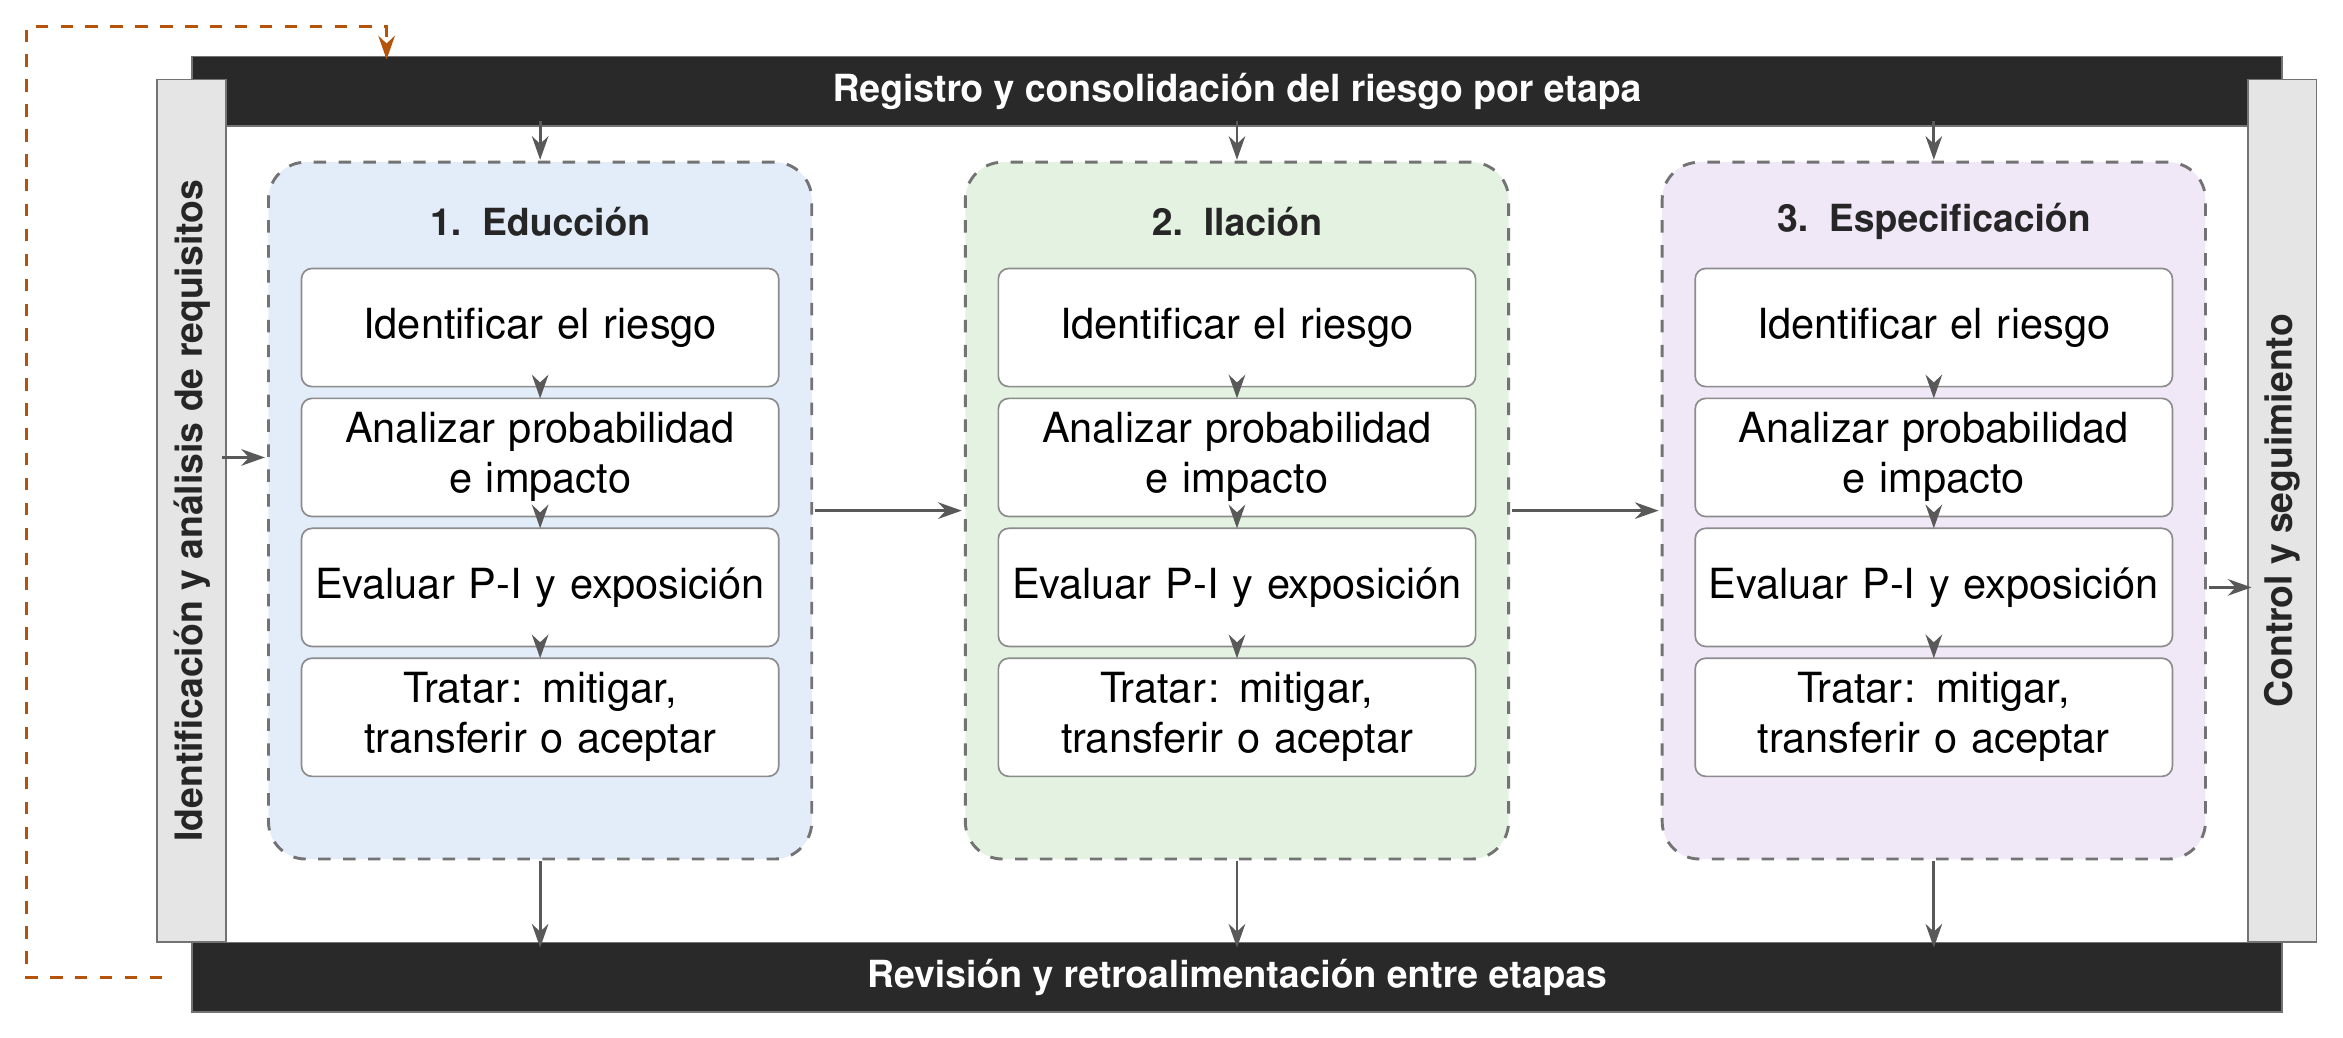
\includegraphics[width=\linewidth]{06-gestion-riesgos.png}
  \caption{Proceso de gestión de riesgos en los requisitos. El ciclo
  identificar, analizar, evaluar y tratar se repite en la educción, la
  ilación y la especificación, dentro de un marco de registro, control y
  retroalimentación que impide aprobar un requisito con un riesgo crítico
  abierto.}
  \label{fig:riesgos-proceso}
\end{figure}

\paragraph{Identificar.} Se revisa cada ficha y cada requisito con una
pregunta única: qué condición incierta podría obligar a rehacerlo. La
respuesta se anota en el registro con el código del requisito, sin valorar
todavía. En esta etapa se apoya en las preguntas abiertas de la
Sección~3.4, en las marcas \texttt{TODO} heredadas de F-02 y en las
discrepancias que la ilación ya dejó documentadas.

\paragraph{Analizar.} Se asigna probabilidad cualitativa y cuantitativa, y
se estima el impacto en jornadas de retrabajo. La estimación se hace por
consenso del equipo y se contrasta con el responsable del requisito.

\paragraph{Evaluar.} Se calcula el índice P-I, se estima el costo por error
y se obtiene la exposición. Con ambos valores se asigna la banda de
severidad y se decide si el riesgo entra en los diez principales.

\paragraph{Tratar.} Se elige una de cuatro respuestas: mitigar (reducir
probabilidad o impacto), transferir (trasladar la responsabilidad, por
ejemplo al contador), aceptar (documentar y monitorear) o evitar (retirar
el requisito del alcance). Cada tratamiento tiene responsable, disparador e
indicador de cierre.

\paragraph{Criterio de salida.} Un requisito no pasa a la línea base
mientras tenga un riesgo crítico abierto. La excepción debe registrarse por
escrito, con el responsable que asume la aceptación.

\subsection{Diseño de la plantilla de trabajo}
\label{subsec:riesgos-plantilla}

\subsubsection{Columnas de la plantilla}
\label{subsubsec:riesgos-columnas}

La plantilla conserva las once columnas del capítulo de referencia y añade,
en el encabezado del registro, los datos de auditoría que el mismo capítulo
propone: código del registro, versión, responsable y fecha de actualización.
La Tabla~\ref{tab:riesgos-columnas} describe cada columna con el ejemplo de
la primera fila del registro.

{\footnotesize\setlength{\tabcolsep}{3pt}
\begin{longtable}{r L{3.0cm} L{7.3cm} L{3.2cm}}
\caption{Columnas de la plantilla de gestión de riesgos.}
\label{tab:riesgos-columnas}\\
\toprule
\textbf{\#} & \textbf{Columna} & \textbf{Qué registra} & \textbf{Ejemplo (R-01)} \\
\midrule
\endfirsthead
\toprule
\textbf{\#} & \textbf{Columna} & \textbf{Qué registra} & \textbf{Ejemplo (R-01)} \\
\midrule
\endhead
\bottomrule
\endfoot
1 & Código requisito & Código de la ficha o del requisito (EDU-, ILA-, RF-, RNF- o R-). & EDU-PRE-05 \\
2 & Riesgo identificado & Enunciado del evento incierto y de su efecto sobre el requisito. & Objeto del prorrateo sin confirmar. \\
3 & Probabilidad (cualitativa) & Etiqueta de la escala de siete niveles. & Muy alta \\
4 & Probabilidad & Porcentaje de ocurrencia, de 0\,\% a 100\,\%. & 95 \\
5 & Impacto & Jornadas de retrabajo si el riesgo ocurre. & 4 \\
6 & Índice P-I & Producto de probabilidad por impacto. & 3,80 \\
7 & Costo por error & Costo de corrección si el error llega a producción. & S/\,1\,800 \\
8 & Exposición al riesgo & Producto del índice P-I por el costo por error. & S/\,6\,840 \\
9 & Estado & Semáforo del tratamiento: resuelto, en proceso, pendiente o retrasado. & en proceso \\
10 & Plan de mitigación & Acción, responsable y condición de cierre del tratamiento. & Sesión con Jerry; acta y V-PRE-02 aprobado. \\
11 & Código artefacto & Artefacto vinculado al requisito (diagrama, interfaz, matriz). & D-02 \\
\end{longtable}
}

\subsubsection{Escalas de probabilidad, impacto y severidad}
\label{subsubsec:riesgos-escalas}

La probabilidad se expresa en una escala de siete niveles para evitar la
falsa precisión de un porcentaje único. La
Tabla~\ref{tab:riesgos-escala-probabilidad} fija la equivalencia y el
criterio de uso; la asignación la hace el equipo y la revisa el responsable
del requisito.

{\small\setlength{\tabcolsep}{4pt}
\begin{longtable}{L{2.6cm} R{1.8cm} L{10.1cm}}
\caption{Escala cualitativa de probabilidad y su equivalencia cuantitativa.}
\label{tab:riesgos-escala-probabilidad}\\
\toprule
\textbf{Nivel} & \textbf{Prob.} & \textbf{Criterio de uso} \\
\midrule
\endfirsthead
\toprule
\textbf{Nivel} & \textbf{Prob.} & \textbf{Criterio de uso} \\
\midrule
\endhead
\bottomrule
\endfoot
Muy baja & 5\,\% & Exigiría un cambio normativo o una decisión externa improbable en el periodo. \\
Baja & 10\,\% & Depende de un tercero que ya confirmó su disponibilidad. \\
Media-baja & 25\,\% & Hay indicios de que la condición puede ocurrir, sin evidencia directa. \\
Media & 50\,\% & La condición es tan probable como su contraria; no hay información para decidir. \\
Media-alta & 75\,\% & La evidencia apunta a que ocurrirá si no se actúa. \\
Alta & 90\,\% & Ya ocurrió en una versión anterior del requisito o en un proyecto similar. \\
Muy alta & 95\,\% & Está ocurriendo ahora mismo y solo falta documentarlo. \\
\end{longtable}
}

El impacto se mide en jornadas de retrabajo y se interpreta con cuatro
tramos: menor (1 a 2 jornadas), moderado (3 a 4), mayor (5 a 6) y severo
(más de 6). El índice P-I resultante se clasifica con los umbrales de la
Tabla~\ref{tab:riesgos-severidad}, que se calibraron sobre la distribución
observada en este registro y no sobre una escala universal.

{\small\setlength{\tabcolsep}{4pt}
\begin{longtable}{L{2.0cm} L{2.2cm} L{6.2cm} L{4.2cm}}
\caption{Bandas de severidad del índice P-I y acción asociada.}
\label{tab:riesgos-severidad}\\
\toprule
\textbf{Banda} & \textbf{Índice P-I} & \textbf{Lectura} & \textbf{Acción} \\
\midrule
\endfirsthead
\toprule
\textbf{Banda} & \textbf{Índice P-I} & \textbf{Lectura} & \textbf{Acción} \\
\midrule
\endhead
\bottomrule
\endfoot
Crítico & 4,5 o más & El riesgo puede consumir una semana o más de retrabajo. & Tratamiento obligatorio antes del cierre de la etapa. \\
Alto & 3,0 a 4,49 & Retrabajo significativo, con impacto en el cronograma. & Tratamiento planificado y seguimiento semanal. \\
Medio & 1,5 a 2,99 & Retrabajo acotado y absorbible. & Seguimiento quincenal. \\
Bajo & menos de 1,5 & Retrabajo menor o poco probable. & Se acepta y se monitorea. \\
\end{longtable}
}

\subsubsection{Semáforo de estado y catálogo de artefactos}
\label{subsubsec:riesgos-semaforo}

El estado del riesgo se representa con los cuatro valores de la
Tabla~\ref{tab:riesgos-estado}. El capítulo de referencia enumera tres
—retrasado, en proceso y pendiente— y usa el verde para el riesgo resuelto;
aquí se incorpora \emph{resuelto} como cuarto valor para poder cerrar el
ciclo y medir el avance del plan.

{\small\setlength{\tabcolsep}{4pt}
\begin{longtable}{L{1.9cm} L{1.7cm} L{6.4cm} L{4.2cm}}
\caption{Estados del riesgo y color asociado.}
\label{tab:riesgos-estado}\\
\toprule
\textbf{Estado} & \textbf{Color} & \textbf{Significado} & \textbf{Qué se hace} \\
\midrule
\endfirsthead
\toprule
\textbf{Estado} & \textbf{Color} & \textbf{Significado} & \textbf{Qué se hace} \\
\midrule
\endhead
\bottomrule
\endfoot
Resuelto & Verde & El tratamiento se aplicó y el indicador de cierre se cumplió. & Se conserva la evidencia y se archiva la fila. \\
En proceso & Amarillo & La acción de mitigación está en ejecución. & Se revisa en la reunión semanal. \\
Pendiente & Gris & El riesgo está identificado y sin acción iniciada. & Se asigna responsable y fecha. \\
Retrasado & Rojo & La acción debía haber cerrado y no ocurrió. & Se escala al responsable del proyecto. \\
\end{longtable}
}

Cada fila del registro se vincula con uno o más artefactos. El
catálogo de la Tabla~\ref{tab:riesgos-artefactos} fija los códigos que se
usan en la columna once y evita que el registro dependa de nombres de
archivo.

{\footnotesize\setlength{\tabcolsep}{3pt}
\begin{longtable}{L{1.4cm} L{6.4cm} L{2.8cm} L{4.0cm}}
\caption{Catálogo de artefactos vinculables a un requisito.}
\label{tab:riesgos-artefactos}\\
\toprule
\textbf{Código} & \textbf{Artefacto} & \textbf{Ubicación} & \textbf{Uso en el registro} \\
\midrule
\endfirsthead
\toprule
\textbf{Código} & \textbf{Artefacto} & \textbf{Ubicación} & \textbf{Uso en el registro} \\
\midrule
\endhead
\bottomrule
\endfoot
D-01 & Venta en mostrador & Figura 1 & Flujo del pedido y del corte \\
D-02 & Abastecimiento y prorrateo & Figura 2 & Reglas de imputación de compras \\
D-03 & Cierre mensual NIIF 18 & Figura 3 & Cascada del resultado y del reporte \\
D-04 & Proceso general del negocio & Figura 4 & Contexto de las tres fases \\
D-05 & Diagrama de clases & Figura 5 & Modelo de datos y reglas de cálculo \\
UI-01 & Carta y pedido del cliente & Figura 6 & Interfaz pública del comensal \\
UI-02 & Mostrador POS & Figura 7 & Operación de caja y controles táctiles \\
UI-03 & Cocina KDS & Figura 8 & Estados del pedido y disponibilidad \\
UI-04 & Dashboard de margen & Figura 9 & Indicadores y ranking de carta \\
UI-05 & Abastecimiento y carta & Figura 10 & Compras, precios y auditoría \\
UI-06 & Cierre NIIF 18 y SUNAT & Figura 11 & Reglas tributarias y comprobantes \\
M-01 & Modelo de datos y reglas de cálculo & Sección 3 & Precisión y redondeo monetario \\
M-02 & Matriz única de requisitos & Tabla 2 & Criterio de aceptación del requisito \\
N-01 & Referencias normativas & F-10 & Reglas tributarias y NIIF 18 \\
T-01 & Tablas de educción e ilación & Sección 2 & Evidencia de la sesión de educción \\
P-01 & Prototipo funcional & Sección 5 & Verificación de la interfaz \\
\end{longtable}
}

\subsection{Resumen del registro}
\label{subsec:riesgos-resumen}

La Tabla~\ref{tab:riesgos-resumen} resume la distribución por etapa y
estado. Los riesgos se codifican con el mismo identificador de la ficha de
origen y se numeran con el prefijo \texttt{R-} para poder citarlos en el
seguimiento. La etapa con mayor exposición acumulada es la especificación,
porque concentra los requisitos que el cliente ya reconoce como propios y,
por tanto, los que más cuesta cambiar.

% =====================================================================
%  riesgos-tabla-resumen.tex — GENERADO AUTOMÁTICAMENTE
%  Fuente: plantillas/registro_riesgos.csv
%  Regenerar con: python3 scripts/generar_riesgos.py  (o make riesgos)
%  No editar a mano: cualquier cambio se pierde al regenerar.
% =====================================================================
{\footnotesize\setlength{\tabcolsep}{3pt}
\begin{longtable}{L{2.0cm} R{1.0cm} R{1.5cm} R{1.4cm} R{1.65cm} R{1.7cm} R{1.8cm} R{2.2cm}}
\caption{Distribución de los riesgos registrados por etapa y estado.}
\label{tab:riesgos-resumen}\\
\toprule
\textbf{Etapa} & \textbf{Total} & \textbf{Resuelto} & \textbf{En proceso} & \textbf{Pendiente} & \textbf{Retrasado} & \textbf{P-I acum.} & \textbf{Exposición acum.} \\
\midrule
\endfirsthead
\toprule
\textbf{Etapa} & \textbf{Total} & \textbf{Resuelto} & \textbf{En proceso} & \textbf{Pendiente} & \textbf{Retrasado} & \textbf{P-I acum.} & \textbf{Exposición acum.} \\
\midrule
\endhead
\bottomrule
\endfoot
Educción & 9 & 0 & 3 & 4 & 2 & 23,95 & 49\,055 \\
Ilación & 8 & 1 & 2 & 5 & 0 & 13,8 & 24\,320 \\
Especificación & 13 & 0 & 5 & 7 & 1 & 31,15 & 62\,040 \\
\midrule
\textbf{Total} & \textbf{30} & \textbf{1} & \textbf{10} & \textbf{16} & \textbf{3} & \textbf{68,9} & \textbf{135\,415} \\
\end{longtable}
}


\subsection{Registro de riesgos por requisito}
\label{subsec:riesgos-registro}

La Tabla~\ref{tab:riesgos-registro} aplica la plantilla de once columnas a
los \RiesgosTotal{} riesgos identificados. Las columnas de cálculo
(\emph{índice P-I} y \emph{exposición}) se generan a partir de la
probabilidad y del impacto, de modo que el registro no puede quedar
internamente inconsistente. El estado se colorea con el semáforo de la
Tabla~\ref{tab:riesgos-estado}.

% =====================================================================
%  riesgos-tabla-registro.tex — GENERADO AUTOMÁTICAMENTE
%  Fuente: plantillas/registro_riesgos.csv
%  Regenerar con: python3 scripts/generar_riesgos.py  (o make riesgos)
%  No editar a mano: cualquier cambio se pierde al regenerar.
% =====================================================================
\begin{landscape}
{\footnotesize\setlength{\tabcolsep}{2pt}\renewcommand{\arraystretch}{1.1}
\begin{longtable}{L{2.2cm} L{4.0cm} L{1.6cm} L{1.0cm} L{1.1cm} L{1.3cm} L{1.3cm} L{2.5cm} L{1.6cm} L{4.8cm} L{1.6cm}}
\caption{Registro de riesgos asociados a los requisitos de RedPepper.}
\label{tab:riesgos-registro}\\
\toprule
\textbf{Código requisito} & \textbf{Riesgo identificado} & \textbf{Prob. cual.} & \textbf{P (\%)} & \textbf{I (días)} & \textbf{Índice P-I} & \textbf{Costo} & \textbf{Exposición} & \textbf{Estado} & \textbf{Plan de mitigación} & \textbf{Artefacto} \\
\midrule
\endfirsthead
\toprule
\textbf{Código requisito} & \textbf{Riesgo identificado} & \textbf{Prob. cual.} & \textbf{P (\%)} & \textbf{I (días)} & \textbf{Índice P-I} & \textbf{Costo} & \textbf{Exposición} & \textbf{Estado} & \textbf{Plan de mitigación} & \textbf{Artefacto} \\
\midrule
\endhead
\bottomrule
\endfoot
\multicolumn{11}{l}{\textbf{Educción de requisitos}} \\
EDU-PRE-05 & El objeto del prorrateo no está confirmado: la solicitud habla de ventas y la aclaración posterior, de compras. El equipo adoptó el reparto de compras como regla candidata. & Muy alta & 95 & 4 & 3,8 & 1\,800 & 6\,840 & \cellcolor{EstadoEnProceso}en proceso & Sesión grabada con Jerry (30 min) para fijar el objeto; congelar la definición en R-PRE-02; actualizar el diagrama 2 con dos casos de prueba (5 y 4 jornadas). & D-02 \\
EDU-PRE-08 & Régimen tributario, tasas y marco contable sin confirmar por el contador; el cálculo de impuestos se apoya en una regla que aún no se aprueba. & Alta & 90 & 6 & 5,4 & 2\,600 & 14\,040 & \cellcolor{EstadoPendiente}pendiente & Acta con el contador con régimen, tributos y vigencia; matriz de reglas por tributo y periodo; versión por fecha de efecto. & N-01 \\
EDU-PRE-10 & El marco de presentación NIIF 18 se declaró como intención del cliente, sin sustento formal de obligatoriedad ni de alcance. & Media & 50 & 5 & 2,5 & 3\,500 & 8\,750 & \cellcolor{EstadoEnProceso}en proceso & Nota de alcance en el acta del proyecto; separar el reporte gerencial con estructura NIIF 18 del cumplimiento acreditado. & D-03 \\
EDU-PRE-14 & El criterio de conciliación entre el reporte mensual y sus comprobantes de sustento no está definido; no hay tolerancia ni partidas de ajuste. & Media & 50 & 3 & 1,5 & 1\,600 & 2\,400 & \cellcolor{EstadoPendiente}pendiente & Definir partidas conciliatorias y tolerancia; incluir el cruce reporte-soporte como criterio de aceptación de RF-14. & UI-06 \\
EDU-OBS-01 & El registro de la observación no consigna fecha, responsables ni duración, de modo que la evidencia no es reproducible. & Media-alta & 75 & 2 & 1,5 & 700 & 1\,050 & \cellcolor{EstadoRetrasado}retrasado & Completar la bitácora de observación con fecha, hora, responsable y duración; adjuntar la evidencia en el repositorio. & T-01 \\
EDU-OBS-05 & El umbral táctil de 48 px es una propuesta del equipo: no se midió en el dispositivo real ni se registró la evidencia. & Media & 50 & 3 & 1,5 & 900 & 1\,350 & \cellcolor{EstadoPendiente}pendiente & Medir el control en el dispositivo aprobado; registrar captura y tabla de tamaños; ajustar RNF-05 si el hardware difiere. & UI-02 \\
EDU-ENT1-01 & La carta no aporta costos unitarios ni recetas, por lo que el ranking y el margen por plato no se pueden calcular con sustento. & Media-alta & 75 & 4 & 3 & 1\,900 & 5\,700 & \cellcolor{EstadoRetrasado}retrasado & Ficha técnica por plato con rendimiento y costo; separar precio de venta de costo directo; validar con Jerry tres platos piloto. & UI-04 \\
EDU-ENT2-14 & El calendario de jornadas hábiles y feriados no está aprobado; el prorrateo puede repartir costos en días no laborados. & Media-alta & 75 & 3 & 2,25 & 1\,300 & 2\,925 & \cellcolor{EstadoEnProceso}en proceso & Calendario oficial del periodo con feriados; regla P-14 documentada; prueba con una semana de cuatro jornadas. & D-02 \\
EDU-ENT2-27 & El alcance de SUNAT es ambiguo: el cliente espera emisión electrónica y el catálogo solo cubre búsqueda y exportación de comprobantes. & Media & 50 & 5 & 2,5 & 2\,400 & 6\,000 & \cellcolor{EstadoPendiente}pendiente & Declarar por escrito que el alcance es búsqueda, filtrado y exportación; registrar la emisión electrónica como fuera de alcance. & UI-06 \\
\multicolumn{11}{l}{\textbf{Ilación de requisitos}} \\
ILA-PRE-02 & Doble contabilización entre el costo directo del producto y la compra semanal prorrateada; ambas bases podrían sumarse en el margen. & Media-alta & 75 & 4 & 3 & 2\,200 & 6\,600 & \cellcolor{EstadoEnProceso}en proceso & Política única de imputación: el prorrateo de compras reemplaza al costo directo en el margen gerencial; prueba de conciliación. & D-02 \\
ILA-PRE-07 & Confusión entre el resultado antes de intereses y el BAI al restar los gastos financieros en un orden incorrecto. & Media & 50 & 2 & 1 & 1\,500 & 1\,500 & \cellcolor{EstadoResuelto}resuelto & Cascada del diagrama 3 corregida: resultado operativo, gastos financieros, BAI e impuesto a la renta en ese orden. & D-03 \\
ILA-PRE-14 & La conciliación mensual no cuenta con una plantilla aprobada; cada versión del reporte usa partidas distintas. & Media & 50 & 4 & 2 & 1\,800 & 3\,600 & \cellcolor{EstadoPendiente}pendiente & Plantilla contable única firmada por el contador; congelar partidas y subtotales antes de codificar. & D-03 \\
ILA-OBS-03 & No se fijó el momento en que la venta queda confirmada (cobro, comanda o entrega); el corte diario puede incluir ventas distintas. & Media & 50 & 3 & 1,5 & 1\,000 & 1\,500 & \cellcolor{EstadoEnProceso}en proceso & Definir la confirmación en el cobro; matriz de estados del pedido; prueba de corte con ventas en distintas etapas. & D-01 \\
ILA-ENT1-01 & La política de producto agotado no existe; carta, POS y cocina podrían tratar el estado de forma distinta. & Media-alta & 75 & 2 & 1,5 & 800 & 1\,200 & \cellcolor{EstadoPendiente}pendiente & Política única: bloqueo en POS y carta, aviso en cocina; caso de prueba con producto marcado como agotado. & UI-02 \\
ILA-ENT2-16 & El recálculo de cuotas al corregir una compra en periodo abierto no tiene regla ni bitácora; las cuotas pueden no sumar el nuevo monto. & Media & 50 & 4 & 2 & 1\,700 & 3\,400 & \cellcolor{EstadoPendiente}pendiente & Regla de recálculo con suma de control; registrar usuario, momento y motivo; prueba de S/ 5\,000 a S/ 500. & UI-05 \\
ILA-ENT2-24 & El ajuste autorizado en un periodo cerrado choca con la inmutabilidad contable; no se definió el asiento de reversión. & Media & 50 & 5 & 2,5 & 2\,500 & 6\,250 & \cellcolor{EstadoPendiente}pendiente & Nota de ajuste firmada con asiento de reversión; bloquear la edición directa y permitir solo el ajuste trazable. & UI-06 \\
ILA-RNF-06 & La regla de redondeo monetario no está definida; DECIMAL(12,4) no indica cuándo ni cómo redondear por moneda. & Baja & 10 & 3 & 0,3 & 900 & 270 & \cellcolor{EstadoPendiente}pendiente & Política de redondeo por moneda y por etapa del cálculo; pruebas de borde con importes de cuatro decimales. & M-01 \\
\multicolumn{11}{l}{\textbf{Especificación de requisitos}} \\
R-PRE-02 & El prorrateo entre jornadas no tiene criterio de aceptación verificable para semanas con feriados o jornadas parciales. & Alta & 90 & 3 & 2,7 & 1\,400 & 3\,780 & \cellcolor{EstadoEnProceso}en proceso & Ampliar V-PRE-02: S/ 500 en cinco jornadas y en cuatro jornadas, cero en feriado y total conservado. & M-02 \\
R-PRE-04 & El margen bruto diario no tiene caso de referencia aprobado; faltan valores esperados para ventas, cuota y adicional. & Media & 50 & 4 & 2 & 1\,500 & 3\,000 & \cellcolor{EstadoPendiente}pendiente & Caso de referencia con ventas S/ 1\,000, cuota S/ 100 y adicional S/ 80 (margen S/ 820); validarlo con Jerry. & D-03 \\
R-PRE-07 & La regla tributaria no se versiona por fecha de efecto; un cambio de tasa podría recalcular periodos anteriores. & Media-alta & 75 & 5 & 3,75 & 2\,800 & 10\,500 & \cellcolor{EstadoEnProceso}en proceso & Versionado por fecha de vigencia y periodo evaluado; prueba con fechas anteriores y posteriores a un cambio autorizado. & UI-06 \\
R-PRE-08 & La plantilla contable mensual no está aprobada; el reporte NIIF 18 puede cambiar de estructura después de la codificación. & Media-alta & 75 & 4 & 3 & 2\,000 & 6\,000 & \cellcolor{EstadoEnProceso}en proceso & Plantilla firmada con partidas, subtotales y totales; congelarla antes de construir el reporte. & D-03 \\
R-ENT2-07 & El reparto entre jornadas efectivamente laboradas no tiene calendario aprobado; feriados y jornadas parciales quedan a interpretación. & Alta & 90 & 3 & 2,7 & 1\,300 & 3\,510 & \cellcolor{EstadoPendiente}pendiente & Calendario aprobado y regla de jornada parcial; prueba de S/ 500 en cuatro jornadas y cero en feriado. & D-02 \\
R-ENT2-10 & La activación de reglas tributarias no exige autorización registrada de Jerry; el contador podría activar un cambio sin control. & Media & 50 & 3 & 1,5 & 1\,900 & 2\,850 & \cellcolor{EstadoPendiente}pendiente & Flujo de aprobación de dos pasos con registro de usuario y fecha; impedir la activación sin autorización. & UI-06 \\
R-ENT2-15 & La compresión de comprobantes no tiene umbral aprobado ni prueba de legibilidad del sustento. & Media & 50 & 2 & 1 & 700 & 700 & \cellcolor{EstadoPendiente}pendiente & Umbral por tamaño y formato; prueba con archivo de referencia y verificación de legibilidad. & UI-05 \\
RF-11 & La parametrización fiscal no cuenta con matriz de reglas por tributo, régimen y periodo; el cálculo queda a criterio del usuario. & Media-alta & 75 & 4 & 3 & 2\,400 & 7\,200 & \cellcolor{EstadoEnProceso}en proceso & Matriz de reglas con vigencia y responsable; el usuario solo selecciona la regla, no edita la tasa. & UI-06 \\
RF-14 & El reporte NIIF 18 no lleva nota de alcance legal y puede interpretarse como acreditación de cumplimiento. & Alta & 90 & 5 & 4,5 & 3\,600 & 16\,200 & \cellcolor{EstadoEnProceso}en proceso & Nota de alcance en el reporte y en el acta; separar la estructura gerencial del cumplimiento acreditado. & UI-06 \\
RF-16 & La búsqueda para SUNAT no tiene criterio de aceptación ni casos de prueba por RUC, fecha y código de gasto. & Media & 50 & 2 & 1 & 800 & 800 & \cellcolor{EstadoPendiente}pendiente & Definir casos de prueba y resultados esperados; validar con el contador tres consultas reales. & UI-06 \\
RF-18 & El dashboard de decisión no tiene indicadores ni umbrales validados; el catálogo de origen no aporta criterio. & Media-alta & 75 & 2 & 1,5 & 900 & 1\,350 & \cellcolor{EstadoRetrasado}retrasado & Definir tres indicadores y sus umbrales con Jerry; acotar el alcance o retirarlo de la línea base. & UI-04 \\
RNF-01 & El control de acceso RBAC no tiene matriz de roles y permisos; cada pantalla define sus permisos por su cuenta. & Media & 50 & 3 & 1,5 & 1\,500 & 2\,250 & \cellcolor{EstadoPendiente}pendiente & Matriz rol por acción; derivar los permisos de la matriz y probar accesos permitidos y denegados. & UI-06 \\
RNF-03 & El umbral de 3 s no tiene dispositivo ni volumen de datos de referencia, por lo que la métrica no es verificable. & Media-alta & 75 & 4 & 3 & 1\,300 & 3\,900 & \cellcolor{EstadoPendiente}pendiente & Benchmark con 12 meses de datos y el dispositivo aprobado; registrar tiempos y percentiles. & UI-02 \\
\end{longtable}
}
\end{landscape}


\subsection{Los diez riesgos principales y el colchón del proyecto}
\label{subsec:riesgos-top10}

La Tabla~\ref{tab:riesgos-top10} ordena los riesgos por índice P-I y, en
caso de empate, por exposición al riesgo. La columna \emph{acumulado} suma
el índice de los riesgos ya ordenados y permite leer cuántas jornadas
aporta cada uno al colchón.

% =====================================================================
%  riesgos-tabla-top10.tex — GENERADO AUTOMÁTICAMENTE
%  Fuente: plantillas/registro_riesgos.csv
%  Regenerar con: python3 scripts/generar_riesgos.py  (o make riesgos)
%  No editar a mano: cualquier cambio se pierde al regenerar.
% =====================================================================
{\footnotesize\setlength{\tabcolsep}{2pt}
\begin{longtable}{R{0.7cm} L{2.2cm} L{4.0cm} R{0.9cm} R{1.1cm} R{1.0cm} R{1.4cm} R{1.9cm} R{1.5cm}}
\caption{Los diez riesgos con mayor índice P-I y su aporte al colchón del proyecto.}
\label{tab:riesgos-top10}\\
\toprule
\textbf{\#} & \textbf{Código} & \textbf{Riesgo (síntesis)} & \textbf{P (\%)} & \textbf{I (días)} & \textbf{P-I} & \textbf{Costo} & \textbf{Exposición} & \textbf{Acum.} \\
\midrule
\endfirsthead
\toprule
\textbf{\#} & \textbf{Código} & \textbf{Riesgo (síntesis)} & \textbf{P (\%)} & \textbf{I (días)} & \textbf{P-I} & \textbf{Costo} & \textbf{Exposición} & \textbf{Acum.} \\
\midrule
\endhead
\bottomrule
\endfoot
1 & EDU-PRE-08 & Régimen y tasas tributarias sin confirmar & 90 & 6 & 5,4 & 2\,600 & 14\,040 & 5,4 \\
2 & RF-14 & Reporte NIIF 18 sin nota de alcance legal & 90 & 5 & 4,5 & 3\,600 & 16\,200 & 9,9 \\
3 & EDU-PRE-05 & Objeto del prorrateo sin confirmar & 95 & 4 & 3,8 & 1\,800 & 6\,840 & 13,7 \\
4 & R-PRE-07 & Regla tributaria sin versionado por fecha & 75 & 5 & 3,75 & 2\,800 & 10\,500 & 17,45 \\
5 & RF-11 & Parametrización fiscal sin matriz de reglas & 75 & 4 & 3 & 2\,400 & 7\,200 & 20,45 \\
6 & ILA-PRE-02 & Doble contabilización del costo directo & 75 & 4 & 3 & 2\,200 & 6\,600 & 23,45 \\
7 & R-PRE-08 & Plantilla contable mensual sin aprobar & 75 & 4 & 3 & 2\,000 & 6\,000 & 26,45 \\
8 & EDU-ENT1-01 & Carta sin costos unitarios ni recetas & 75 & 4 & 3 & 1\,900 & 5\,700 & 29,45 \\
9 & RNF-03 & Umbral de 3 s sin referencia de medición & 75 & 4 & 3 & 1\,300 & 3\,900 & 32,45 \\
10 & R-PRE-02 & Prorrateo sin criterio de aceptación verificable & 90 & 3 & 2,7 & 1\,400 & 3\,780 & 35,15 \\
\midrule
\multicolumn{8}{r}{\textbf{Colchón de exposición bruta (suma P-I)}} & \textbf{35,15} \\
\end{longtable}
}


\paragraph{Lectura del ranking.} Los diez riesgos principales concentran el
51\,\% del índice P-I total del registro. El patrón es claro y tiene tres
bloques. El primero es tributario-contable: el régimen sin confirmar, la
nota de alcance de NIIF 18, el versionado de la regla por fecha y la matriz
de parametrización ocupan cuatro de los cinco primeros puestos. El segundo
es el prorrateo y el costo: el objeto del prorrateo, la doble
contabilización y el criterio de aceptación del reparto. El tercero es la
base documental: la plantilla contable, los costos unitarios de la carta y
la medición de rendimiento.

\paragraph{El colchón.} El colchón de exposición bruta se calcula como la
suma de los índices P-I de los diez riesgos principales:

\[
\mbox{Colchón} = \sum_{i=1}^{10} P_i \times I_i = \ColchonBruto\ \mbox{jornadas}
\]

Sobre un cronograma de referencia de \JornadasProyecto{} jornadas (16
semanas de lunes a viernes), ese valor equivale al \ColchonPorcentaje\,\%.
No es un plazo que deba añadirse al cronograma: es la exposición esperada
si no se actúa. Con la mitigación prevista, la probabilidad residual de los
diez riesgos baja y el colchón se reduce a \ColchonResidual{} jornadas
(\ColchonResidualPorcentaje\,\%), es decir, \ColchonAhorro{} jornadas menos.
La recomendación para la revisión es reservar el colchón residual
(\ColchonResidual{} jornadas) como reserva de contingencia y liberar cinco
jornadas adicionales como reserva de gestión, revisando ambas al cierre de
cada etapa.

\paragraph{Qué no dice el colchón.} El índice P-I no distingue entre riesgos
que ocurren en paralelo y riesgos que se suman; tampoco incorpora el costo
financiero del retraso ni el efecto de un riesgo sobre otro. Es una
herramienta de priorización, no una predicción. Su valor está en comparar y
ordenar, y en obligar a que cada riesgo tenga un responsable y una condición
de cierre.

\subsection{Plan de mitigación y seguimiento}
\label{subsec:riesgos-plan}

La Tabla~\ref{tab:riesgos-plan} desarrolla el tratamiento de los diez
riesgos principales: acción, responsable, disparador que activa la acción,
indicador de cierre y probabilidad residual estimada una vez aplicada la
mitigación.

% =====================================================================
%  riesgos-tabla-plan.tex — GENERADO AUTOMÁTICAMENTE
%  Fuente: plantillas/registro_riesgos.csv
%  Regenerar con: python3 scripts/generar_riesgos.py  (o make riesgos)
%  No editar a mano: cualquier cambio se pierde al regenerar.
% =====================================================================
\begin{landscape}
{\footnotesize\setlength{\tabcolsep}{3pt}\renewcommand{\arraystretch}{1.1}
\begin{longtable}{L{2.4cm} L{3.0cm} L{5.5cm} L{2.3cm} L{3.3cm} L{3.5cm} R{1.6cm}}
\caption{Plan de mitigación y seguimiento de los diez riesgos principales.}
\label{tab:riesgos-plan}\\
\toprule
\textbf{Código} & \textbf{Riesgo} & \textbf{Acción de mitigación} & \textbf{Responsable} & \textbf{Disparador} & \textbf{Indicador de cierre} & \textbf{P res. (\%)} \\
\midrule
\endfirsthead
\toprule
\textbf{Código} & \textbf{Riesgo} & \textbf{Acción de mitigación} & \textbf{Responsable} & \textbf{Disparador} & \textbf{Indicador de cierre} & \textbf{P res. (\%)} \\
\midrule
\endhead
\bottomrule
\endfoot
EDU-PRE-08 & Régimen y tasas tributarias sin confirmar & Acta con el contador con régimen, tributos y vigencia; matriz de reglas por tributo y periodo; versión por fecha de efecto. & Contador / Jerry & El contador no entrega la regla antes del cierre & Matriz de reglas firmada & 45 \\
RF-14 & Reporte NIIF 18 sin nota de alcance legal & Nota de alcance en el reporte y en el acta; separar la estructura gerencial del cumplimiento acreditado. & Jerry & El cliente presenta el reporte ante SUNAT & Nota de alcance visible & 40 \\
EDU-PRE-05 & Objeto del prorrateo sin confirmar & Sesión grabada con Jerry (30 min) para fijar el objeto; congelar la definición en R-PRE-02; actualizar el diagrama 2 con dos casos de prueba (5 y 4 jornadas). & Jerry / Gabriel Pajuelo & Jerry no confirma en la revisión & Acta firmada y V-PRE-02 aprobado & 40 \\
R-PRE-07 & Regla tributaria sin versionado por fecha & Versionado por fecha de vigencia y periodo evaluado; prueba con fechas anteriores y posteriores a un cambio autorizado. & Contador & Cambio de tasa a mitad de periodo & Versión correcta en la prueba & 30 \\
RF-11 & Parametrización fiscal sin matriz de reglas & Matriz de reglas con vigencia y responsable; el usuario solo selecciona la regla, no edita la tasa. & Contador & Usuario edita una tasa directamente & Matriz aprobada y bloqueo de edición & 30 \\
ILA-PRE-02 & Doble contabilización del costo directo & Política única de imputación: el prorrateo de compras reemplaza al costo directo en el margen gerencial; prueba de conciliación. & Gabriel Pajuelo & El margen difiere del caso de referencia & Conciliación sin doble conteo & 30 \\
R-PRE-08 & Plantilla contable mensual sin aprobar & Plantilla firmada con partidas, subtotales y totales; congelarla antes de construir el reporte. & Contador & Nueva estructura en la revisión & Plantilla 1.0 congelada & 30 \\
EDU-ENT1-01 & Carta sin costos unitarios ni recetas & Ficha técnica por plato con rendimiento y costo; separar precio de venta de costo directo; validar con Jerry tres platos piloto. & Jerry / José Chino & El cliente no entrega recetas & Tres fichas técnicas aprobadas & 35 \\
RNF-03 & Umbral de 3 s sin referencia de medición & Benchmark con 12 meses de datos y el dispositivo aprobado; registrar tiempos y percentiles. & José Choquehuanca & El cierre tarda más de 3 s en el local & Benchmark documentado & 30 \\
R-PRE-02 & Prorrateo sin criterio de aceptación verificable & Ampliar V-PRE-02: S/ 500 en cinco jornadas y en cuatro jornadas, cero en feriado y total conservado. & Gabriel Pajuelo & Semana con feriado en el caso de prueba & V-PRE-02 aprobado con dos casos & 35 \\
\end{longtable}
}
\end{landscape}


\paragraph{Ritmo de seguimiento.} El registro se revisa en una reunión
semanal de veinte minutos con el responsable de cada riesgo abierto. En cada
revisión se actualiza el estado, se registra la fecha y la nota en la
columna de auditoría y se recalculan el índice y el colchón. Al cierre de
cada etapa se presenta el resumen a Jerry y al contador, con los riesgos
críticos y las decisiones que dependen de ellos.

\paragraph{Indicadores del plan.} Se siguen cuatro indicadores: porcentaje
de riesgos cerrados sobre el total, variación del colchón respecto de la
línea base, número de mitigaciones retrasadas y exposición acumulada de los
riesgos críticos. El primero mide avance; el segundo, eficacia; el tercero,
disciplina; el cuarto, riesgo residual.

\paragraph{Escalamiento.} Un riesgo crítico sin tratamiento al cierre de la
etapa se escala al responsable del proyecto y se registra como excepción
firmada. Un riesgo retrasado dos semanas consecutivas se escala al docente
y al cliente. Un riesgo que cambia de banda de severidad se renegocia con
el responsable del requisito antes de la siguiente revisión.

\subsection{Estado del avance, limitaciones y decisiones para la revisión}
\label{subsec:riesgos-estado}

\paragraph{Lo que está hecho.} El registro cubre las tres etapas con
\RiesgosTotal{} riesgos, de los cuales \RiesgosCriticos{} son críticos y
\RiesgosAltos{} altos. Los diez principales tienen plan de mitigación con
responsable, disparador e indicador de cierre. El cálculo del índice, de la
exposición y del colchón es reproducible: se regenera desde el archivo de
datos con un comando y no se edita a mano.

\paragraph{Lo que falta.} La cuantificación es preliminar y debe validarse
en tres frentes: una ronda de juicio experto con el equipo para confirmar
probabilidades e impactos; una revisión de los costos por error con el
contador; y la asignación de fechas comprometidas a cada mitigación. Además,
treinta y siete requisitos del catálogo no tienen un riesgo asociado, lo que
no significa que estén libres de riesgo: significa que el equipo no
identificó uno en esta primera pasada y debe declararlo así.

\paragraph{Limitaciones.} Los valores no provienen de un histórico de
proyectos. El costo por error se estima con el criterio de que un defecto
detectado en producción cuesta entre diez y veinte veces más que uno
detectado en requisitos, pero no se aplicó un factor formal por etapa. El
colchón es una heurística de priorización y no reemplaza al plan de riesgos
del proyecto completo, que debe cubrir cronograma, presupuesto, proveedores
y personal. La moneda es el sol peruano y los importes no incluyen IGV.

\paragraph{Decisiones que se solicitan en la revisión.} Aprobar la escala de
probabilidad y los umbrales de severidad; aprobar la plantilla de once
columnas y el catálogo de artefactos; validar los diez riesgos principales y
sus responsables; fijar la fecha de la primera revisión semanal; y autorizar
la conversión de los riesgos tributarios en requisitos de calidad
verificables, con el contador como responsable de la regla.

\paragraph{Cierre.} La lección del capítulo de referencia se cumple en este
caso: los riesgos de requisitos no se evitan, se transforman. El objeto del
prorrateo, la vigencia de la regla tributaria y la nota de alcance de NIIF 18
dejan de ser supuestos y pasan a ser requisitos con criterio de aceptación.
Ese es el resultado que el plan persigue y el que la revisión debe confirmar.
